\documentclass{article}
\usepackage{amsmath,graphicx}
\usepackage{cite}
\usepackage{amsthm,amssymb,amsfonts}
\usepackage{textcomp}
\usepackage{bm,enumerate}
\usepackage{algorithm}    
\usepackage{algorithmic}
\usepackage{booktabs}
\usepackage{dsfont}

\renewcommand{\algorithmicrequire}{ \textbf{Input:}}     
\renewcommand{\algorithmicensure}{ \textbf{Output:}}
\renewcommand{\mathbf}{\boldsymbol}
\newcommand{\mb}{\mathbf}
\newcommand{\matlab}[1]{\texttt{#1}}
\newcommand{\setname}[1]{\textsl{#1}}
\newcommand{\Ce}{\mathbb{C}}
\newcommand{\Ee}{\mathbb{E}}
\newcommand{\Ne}{\mathbb{N}}
\newcommand{\Se}{\mathbb{S}}
\newcommand{\norm}[2]{\left\| #1 \right\|_{#2}}

\DeclareMathOperator*{\minimize}{minimize}

\begin{document}

\title{Machine Learning, Spring 2018\\Homework 3}
\date{Due on 23:59 Apr 17, 2018\\Send to $cs282\_01@163.com$ \\with subject "Chinese name+student number+HW3"}
\maketitle




\section{Perceptron}


\begin{enumerate}[(1)]
\item 
\begin{proof}
$\because \bm{w}(t+1) \leftarrow \bm{w}(t) + y(t)\bm{x}(t)$, we have\\
% \bm{x}(t)$ is misclassified by $\bm{w}(t)$so$y(t)\bm{w^T}(t)\bm{x}(t)<0$:\\
% $\bm{w}(t+1)$ correctly classifies $\bm{x}(t)$ so $y(t)\bm{w^T}(t+1)\bm{x}(t)>0$\\
% Hence:$y(t)\bm{w^T}(t+1)\bm{x}(t)>y(t)\bm{w^T}(t)\bm{x}(t)$
% $y(t)=+1$: $sign(\bm{w^T}(t)\bm{x}(t))=-1\LeftRightarrow\bm{w^T}(t)\bm{x}(t)<0$.Hence:$y(t)\bm{w^T}(t)\bm{x}(t)<0$\\
\begin{equation}
\begin{aligned}
y(t)\bm{w^T}(t+1)\bm{x}(t) &= y(t)[\bm{w^T}(t) + y(t)\bm{x^T}(t)]\bm{x}(t)\\
&=y(t)\bm{w^T}(t)\bm{x}(t) + |y(t)|\norm{\bm{x}(t)}{2}\\
&\geq y(t)\bm{w^T}(t)\bm{x}(t)
\end{aligned}
\end{equation}

Since, $\bm{x}(t)$ is misclassified by $\bm{w}(t)$\\
$\therefore y(t)\bm{w^T}(t)\bm{x}(t)<0$\\
So, we have $\norm{\bm{x}(t)}{2}\neq 0$\\
Therefore, $y(t)\bm{w^T}(t+1)\bm{x}(t)>y(t)\bm{w^T}(t)\bm{x}(t)$.
\end{proof}
\item Suppose $\bm{x}(t)$ was misclassified.\\
$\because \bm{w}(t+1) \leftarrow \bm{w}(t) + y(t)\bm{x}(t)$, we have\\
$\bm{w^T}(t+1)\bm{x}(t) = \bm{w^T}(t)\bm{x}(t) + y(t)(\bm{x}(t)\cdot \bm{x}(t))$\\

If $\bm{x}(t)$ was incorrectly classified as negative, then $y(t) = +1$. It follows that the new dot product increased by $\bm{x}(t)\cdot \bm{x}(t)$ (which is positive). The boundary moved in the right direction as far as $\bm{x}(t)$ is concerned, therefore.\\
Conversely, if $\bm{x}(t)$ was incorrectly classified as positive, then $y(t) = -1$. It follows that the new dot product decreased by $\bm{x}(t)\cdot \bm{x}(t)$ (which is positive). The boundary moved in the right direction as far as $\bm{x}(t)$ is concerned, therefore.
\end{enumerate}



\section{Understanding logistic regression}


\textbf{Answer}: 
\begin{enumerate}[(1)]
	\item Suppose $p = \mathbb{P}(\bm{y}=1|\bm{x})$\\
	\begin{equation}
	\begin{aligned}
	 \text{logit}(p) &= \log \frac{p}{1-p} = \bm{w^T}\bm{x^{(i)}}\\
	 p &= \frac{1}{1+e^{\bm{w^T}\bm{x^{(i)}}}}\\
	 &=\sigma(\bm{w}^T\bm{x^{(i)}})
	\end{aligned}
	\end{equation}
	% =\sigma(\bm{w}^T\bm{x})$. (Hint: The conception \emph{odd ratio} may be helpful.) (5 points)
	% \item The MSE for logistic regression, i.e., 
	% $$J(\bm{w}) = \frac{1}{m} \sum_{i=1}^{m}(\sigma(\bm{w}^T\bm{x}^{(i)})-y^{(i)})^2.$$
	% is not a good loss function. Why? (5 points)
	\item As long as $\bm{x}$ is not zero, the squared error loss with respect to $\bm{w}$ will be non-convex. It's hard to optimize. Whereas the log loss is convex.

	% \item Now suppose we have a 3-class task, i.e., $y(i)\in\{1,2,3\}$, find the Negative Log-Likelyhood of the given data (the objective of the softmax regression problem). (10 points)
	\item $$\mathbb{P}(y^{(i)}=k|\bm{x}=\bm{x}^{(i)}) = \mathds{1}\{y^{(i)}=k\}\frac{e^{f_{y^{(i)}}}}{\sum_{j=1}^{3}e^{f_j}}$$\\
	in there $f(\bm{x}^{(i)}, \bm{W})=\bm{W}^T\bm{x}^{(i)}$,$k=1,2,3$\\
	$$L(y^{(1)},\dots,y^{(N)}|\bm{x}^{(1)},\dots, \bm{x}^{(N)};\bm{W}) = \prod_{i=1}^{N}\mathds{1}\{y^{(i)}=k\}\frac{e^{f_{y^{(i)}}}}{\sum_{j=1}^{3}e^{f_j}}$$\\
	The Negative Log-Likelyhood of the $N$ samples as follows:\\
	$$-\ln{L} = -\sum_{i=1}^{N}\mathds{1}\{y^{(i)}=k\}(f_{y^{(i)}}-\ln{\sum_{j=1}^{3}e^{f_j}})$$
\end{enumerate}



\section{Regularization}

% The goal in the prediction problem is to be able to make prediction for the target variable $t$ given some new value of the input variable $x$ on the basis of a set of training data comprising $N$ input values $\textbf{x} = (x_1,\dots,x_N)^T$ and their corresponding target variable $\textbf{t}= (t_1,\dots,t_N)^T$. we could assume that, given the value of x , the corresponding value of $t$ has a Guassian distribution with a mean equal to the value $y(x,w)$ and the variance $\sigma$, where $y(x,w)$ is the prediction function. For example, for the linear regression, the $y(x,\textbf{w}) = w_0+w_1x$.

% Thus, we have \[p(t|x,\textbf{w}, \sigma) = \mathcal{N}(t|y(x,\textbf{w}),\sigma)\]
% Here we only consider the case of a single real-valued variable $x$.
% Now  you need  to use the training data $\{\textbf{x},\textbf{t}\}$ to determine the parameter $\textbf{w}$ and $\sigma$ by maximum likelihood. 
\begin{enumerate}[(1)]
	% \item Show that maximizing the log likehood is equal to minimizing the sum-of-squares error function. (10 points)
	\item 
	\begin{proof}
	For sigle sample:\\

	$$p(t|x,\textbf{w}, \sigma) = \frac{1}{\sqrt{2\pi}\sigma}e^{-\frac{[t-y(x,\textbf{w})]^2}{2\sigma^2}}$$\\
	For all samples, likehood is :\\
	$$L = \prod_{i=1}^{N} p(t_i|x_i,\bm{w}, \sigma) = \prod_{i=1}^{N}\frac{1}{\sqrt{2\pi}\sigma}e^{-\frac{(t_i-y_i)^2}{2\sigma^2}}$$\\
	log-likehood: \\
	$$\ln{L} = -N\ln{\sqrt{2\pi}\sigma}-\frac{1}{2\sigma^2}\sum_{i=1}^{N}(t_i-y_i)^2$$\\
	$\therefore$ Maximizing the log likehood is equal to minimizing the sum-of- squares error function.
	\end{proof}
	% \item More, if we assume that the ploynomial codfficients $\textbf{w}$ is distributed as the Guassian distribution of the form
	% \[p(\textbf{w}|\alpha) =  \mathcal{N}(\textbf{w}|\textbf{0},\alpha \textbf{I})\]
	% where $\alpha$ is the paramater of the distribution.
	% Then what is the formulation of the prediction problem?  And give us the regularization parameter. Please show us the induction of the procedure.\\
	% (Hint. Using Bayes' theorem) (15 points)
	\item 
	According to Bayes' theorem, for sigle sample:\\
	\begin{equation}
	\begin{aligned}
	p(t,\bm{w}|x, \alpha, \sigma) &= p(t|\bm{w}, x,\alpha, \sigma)\cdot p(\bm{w}|x,\alpha, \sigma)\\
	&=\frac{1}{\sqrt{2\pi}\sigma}e^{-\frac{[t-y(x,\textbf{w})]^2}{2\sigma^2}}\cdot \frac{1}{\sqrt{(2\pi)^D|\alpha I|}}e^{-\frac{1}{2}\bm{w}^T(\alpha I)^{-1}\bm{w}}\\
	&=\frac{1}{\sqrt{2\pi}\sigma}e^{-\frac{[t-y(x,\textbf{w})]^2}{2\sigma^2}}\cdot \frac{1}{\sqrt{(2\pi\alpha)^D}}e^{-\frac{1}{2\alpha}\norm{\bm{w}}2}
	\end{aligned}
	\end{equation}
	For all samples, likehood is :\\
	\begin{equation}
		\begin{aligned}
		L &= {\displaystyle \prod_{i=1}^{N}} p(t_i,\bm{w}|x_i,\alpha,\sigma)\\
		&=(\frac{1}{\sqrt{2\pi}\sigma})^N(\frac{1}{\sqrt{(2\pi\alpha)^D}})^N exp({\displaystyle \sum_{i=1}^{N}}(-\frac{1}{2\sigma^2}(t_i-y_i)^2 - \frac{1}{2\alpha}\norm{\bm{w}}2)
		\end{aligned}
	\end{equation}
	$\frac{1}{N}$log-likehood: \\
	$$\frac{1}{N}\ln{L} = C - \frac{1}{N}{\displaystyle \sum_{i=1}^{N}}(\frac{1}{2\sigma^2}(t_i-y_i)^2 + \frac{1}{2\alpha}\norm{\bm{w}}2), C \text{ is constant}$$
	The formulation of the prediction problem is:\\
	$$\displaystyle{\minimize\frac{1}{N}{\displaystyle \sum_{i=1}^{N}}(\frac{1}{2\sigma^2}(t_i-\bm{w}^Tx_i))^2 + \frac{1}{2\alpha}\norm{\bm{w}}2)}$$
\end{enumerate}


\section{Program Logistic regression in matlab} 
% Program a matlab function based on the algorithms (Negative gradient, Newton's direction, and BFGS) you have learned 
% \begin{verbatim}
% [weight, gradnormList] = logisticRegression(X, y),
% \end{verbatim}
% where $\mb{X}$ is the data matrix and $\mb{y}$ is the label. You may like to read the matlab script \matlab{hw3\_demo.m} first and following the description in it.
\begin{enumerate}[(1)]
% \item The first case is a very simple dataset given as follows
% \begin{equation}
% \begin{bmatrix}
% 0 & 0 & 0 \\
% 2 & 2 & 0\\
% 2 & 0 & +1\\
% 3 & 0 & +1
% \end{bmatrix}
% \end{equation}
% where the first two columns are the attributes (data matrix $\mb{X}$) and the last column is the label $\mb{y}$. Plot the norm of gradient corresponding to three algorithms to illustrate the convergence. (10 points)
\item Fig.1. shows the norm of gradient corresponding to three algorithms. All of three algorithms were terminated when the norm of gradient small than 0.00001(In last question, I change it to 0.001 for BFGS and add normalization, so plot maybe different as shown.) and keep in one Matlab function file named $lr\_lindq.m$. Each algorithm was called by a extra arguments $type$, 0, 1 and 2 corresponding to Negative gradient, Newton’s direction and BFGS, respectively.
\begin{figure}[htb]
\centering
  \begin{tabular}{@{}ccc@{}}
    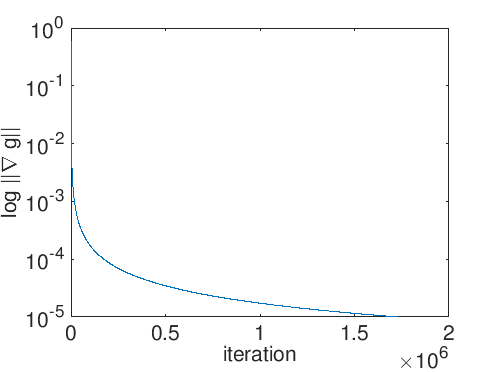
\includegraphics[width=.33\textwidth]{hw3_0.png} &
    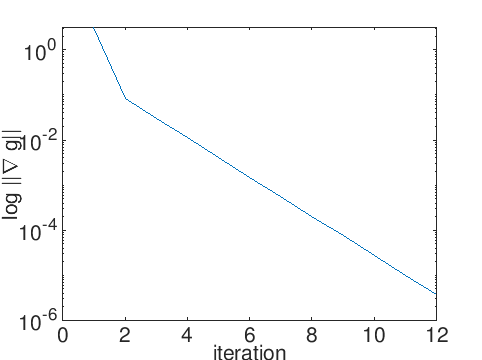
\includegraphics[width=.33\textwidth]{hw3_1.png} &
    % \includegraphics[width=.2\textwidth]{2092.png} &
    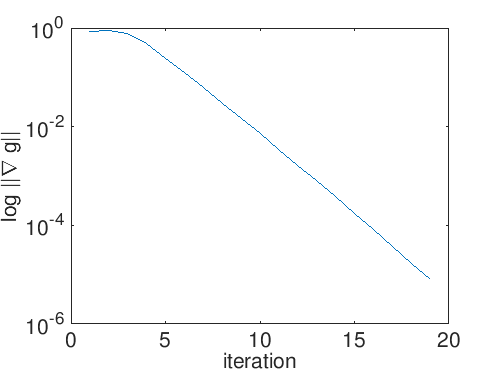
\includegraphics[width=.33\textwidth]{hw3_2.png}   \\
    % \multicolumn{3}{c}{\includegraphics[width=.2\textwidth]{2092.png}}
  \end{tabular}
  \caption{Negative gradient(left), Newton’s direction(middle) and BFGS(right)}
\end{figure}

% \item Run your function on \matlab{nbadata.mat} dataset based on BFGS and compute the accuracy of prediction in training set. (15 points)
\item Terminate the BFGS when the norm of gradient small than $0.001$. Accuracy of prediction in training set is equal to $0.9699$.
% \item The dataset \matlab{nbadata.mat} is class-imbalance. Modifying your algorithm (again, based on BFGS) that enable it to be applied to the situation of class-imbalance and compute the accuracy of prediction in training set. (Please give a detailed description of your methods and explain why in report.) (15 points)
\item Consider very small amount of champion data, I amplified some entries in Hessian matrix relate to champion data. Since $H=X^TDX$, I zoomed in the entries in $D$ with 20000x, where is champion data, say $y_i = 1$. Terminate the BFGS when the norm of gradient small than $0.001$. Accuracy of prediction in training set is equal to $0.9725$.
See code in $lr\_lindq.m$ when $type=3$.
\end{enumerate}



\end{document}